% Created 2023-03-20 Mon 13:48
% Intended LaTeX compiler: lualatex
\documentclass[bigger]{beamer}
\usepackage{graphicx}
\usepackage{longtable}
\usepackage{wrapfig}
\usepackage{rotating}
\usepackage[normalem]{ulem}
\usepackage{amsmath}
\usepackage{amssymb}
\usepackage{capt-of}
\usepackage{hyperref}
\usetheme[progressbar=foot, sectionpage=none, numbering=fraction]{metropolis}
\usepackage{tikz}
\usepackage{booktabs}
\usepackage{adjustbox}
\usepackage{diagbox}
\usepackage{latexcolors}
\usetikzlibrary{automata, positioning, arrows, arrows.meta}
\usepackage{diagbox}
\usepackage{dsfont}
\usepackage{amsmath}
\usepackage{fontawesome5}
\usepackage{color}
\usepackage{transparent}
\definecolor{RedBrown}{RGB}{192, 4, 4} \setbeamercolor{progress bar}{fg=RedBrown} \setbeamercolor{title separator}{fg=RedBrown}
\setbeamercolor{progress bar in head/foot}{fg=RedBrown} \setbeamercolor{progress bar in section page}{fg=RedBrown} \setbeamercolor{alerted text}{fg=RedBrown}
\pretocmd{\tableofcontents}{\thispagestyle{empty}}{}{}
\addtocounter{framenumber}{-1}
\usepackage{listings}
\usepackage{xcolor}
\definecolor{codegreen}{rgb}{0,0.6,0}
\definecolor{codegray}{rgb}{0.5,0.5,0.5}
\definecolor{codepurple}{rgb}{0.58,0,0.82}
\definecolor{backcolour}{HTML}{f0f0f0}
\lstdefinestyle{mystyle}{
backgroundcolor=\color{backcolour},
commentstyle=\color{codegreen},
keywordstyle=\color{magenta},
numberstyle=\tiny\color{codegray},
stringstyle=\color{codepurple},
basicstyle=\ttfamily,
breakatwhitespace=false,
breaklines=true,
captionpos=b,
keepspaces=true,
numbers=none,
numbersep=5pt,
showspaces=false,
showstringspaces=false,
showtabs=false,
tabsize=2
}
\lstset{style=mystyle}
\usetheme{default}
\author{Andrea Pierré}
\date{April 4\textsuperscript{th}, 2023}
\title{NSGP seminar}
\subtitle{Learning useful representations to solve a place-odor association task}
\institute{Brown University}
\titlegraphic{\hfill
\includegraphics[height=1.5cm]{img/Brown Logo_2016_2 Color Process ST_1300.png}}
\setbeamercovered{transparent=10}
\setbeamertemplate{section in toc}[sections numbered]
\AtBeginSection[]{\begin{frame}[plain, noframenumbering]{Outline}    \setbeamertemplate{section in toc}[sections numbered]\setbeamertemplate{subsection in toc}[subsections numbered]\tableofcontents[currentsection, currentsubsection]\end{frame}}
\AtBeginSubsection[]{\begin{frame}[plain, noframenumbering]{Outline}\setbeamertemplate{section in toc}[sections numbered]\setbeamertemplate{subsection in toc}[subsections numbered]\tableofcontents[currentsection,currentsubsection]\end{frame}}
\begin{document}

\maketitle
\begin{frame}[plain]{Outline}
\tableofcontents
\end{frame}

\section{Context}
\label{sec:orgff87777}
\begin{frame}[label={sec:orge12060c}]{Context}
\end{frame}
\begin{frame}[label={sec:orgd08aaca}]{Rationale}
\begin{block}{Why we record in the LEC?}
\end{block}
\end{frame}
\begin{frame}[label={sec:org594741b}]{Joint representation}
\end{frame}
\begin{frame}[label={sec:orga0dd99b}]{What is Reinforcement Learning and why we want to use it ?}
\begin{columns}
\begin{column}{0.6\columnwidth}
% \usepackage{fontawesome5}
\usetikzlibrary{positioning,fit,arrows}


\tikzset{
    %Define standard arrow tip
    >=latex,
    %Define style for boxes
    punkt/.style={
           rectangle,
           rounded corners,
           draw=black, very thick,
           text width=7.5em,
           minimum height=2em,
           text centered},
    % Define arrow style
    pil/.style={
           ->,
           thick,}
}

\begin{adjustbox}{max width=\columnwidth, keepaspectratio}
    \begin{tikzpicture}[node distance=3em, auto,]
     %nodes
        \node (center) {};
        \node[punkt, above=of center] (agent) {Agent \faIcon{robot}};
        \node[punkt,below=of center] (environment) {Environment \faIcon{globe}};
        \node[right=8em of center, align=center] (action) {Action\\$a_t$};
        \node[left=8em of center, align=center] (state_reward) {State, Reward\\$s_t$, $r_t$};

        \path[pil]
        (state_reward.east) edge [->, bend left=45] node {} (agent.west)
        (environment.west) edge [- , bend left=45] node {} (state_reward.east)
        (action.west) edge [->, bend left=45] node {} (environment.east)
        (agent.east) edge [-, bend left=45] node {} (action.west);
    \end{tikzpicture}
\end{adjustbox}
\end{column}

\begin{column}{0.4\columnwidth}
\small
\begin{itemize}
\item Goal of the agent : maximize rewards
\item Natural fit for behavioral experiments involving rewards and learning
\end{itemize}
\end{column}
\end{columns}
\end{frame}

\section{Experimental setup and task}
\label{sec:org97c4284}
\begin{frame}[label={sec:org5124494}]{Olivia's diamond arena olfactory task}
\begin{columns}
\begin{column}[t]{0.5\columnwidth}
\center
Allocentric\\
(go west/east)
\begin{center}
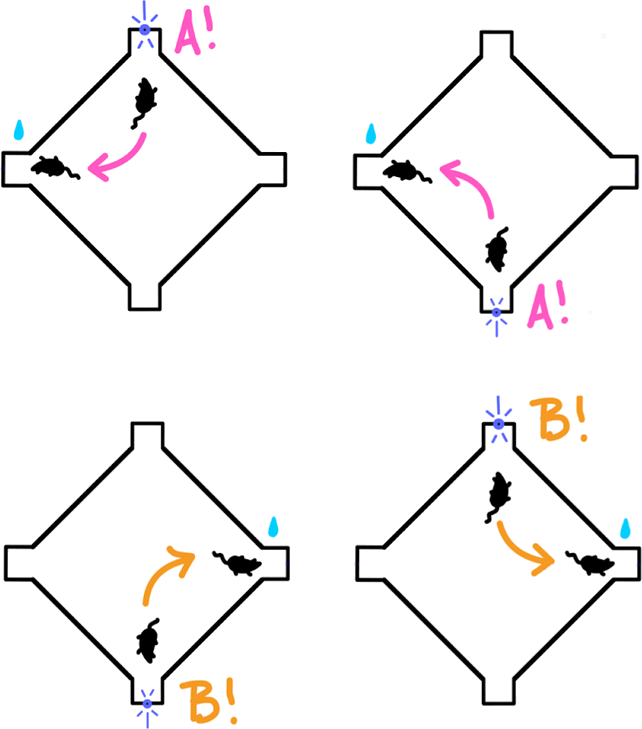
\includegraphics[width=0.8\textwidth]{img/allocentric-task.png}
\end{center}
\end{column}

\begin{column}[t]{0.5\columnwidth}
\center
Egocentric\\
(go right/left)
\begin{center}
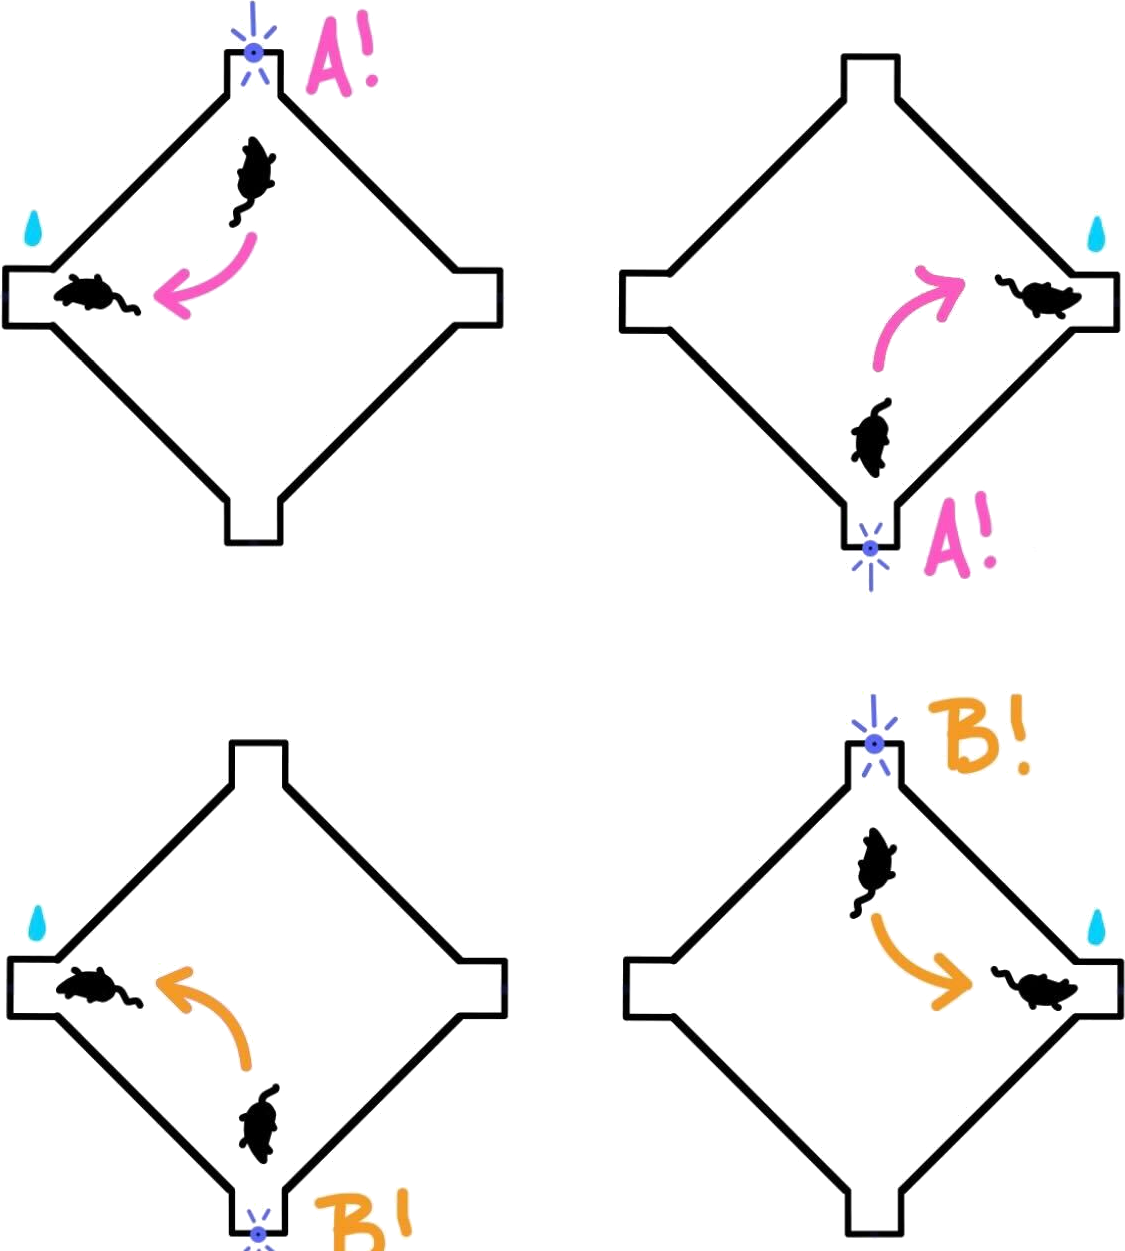
\includegraphics[width=0.8\textwidth]{img/egocentric-task.png}
\end{center}

\begin{textblock}{5}(-1,13)
\center
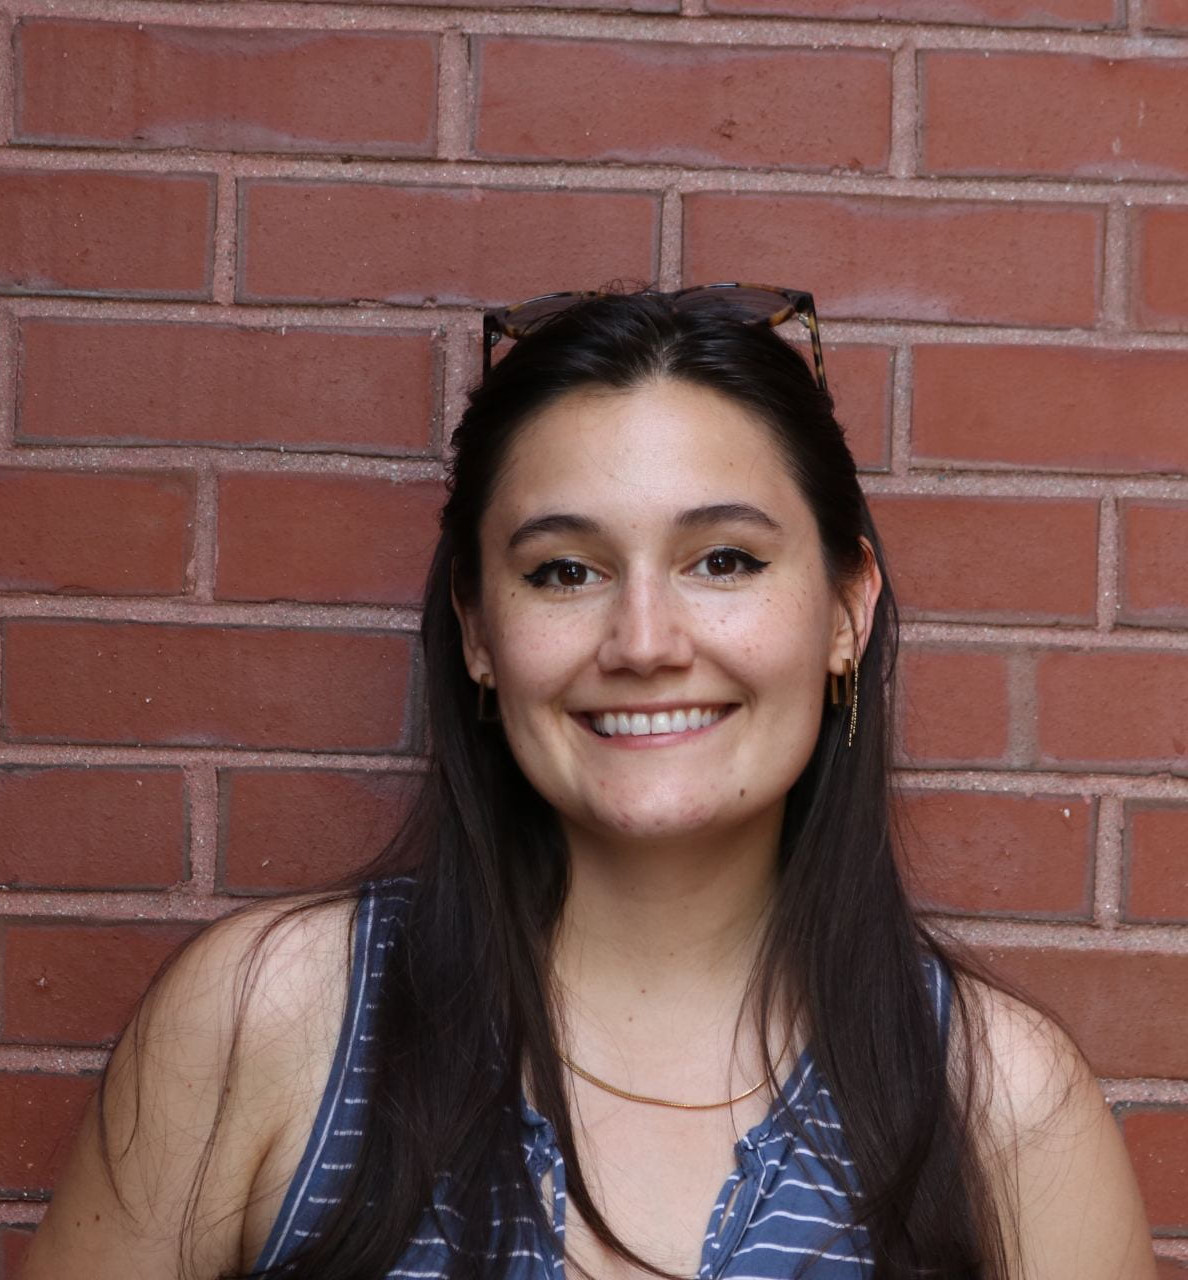
\includegraphics[width=3em]{img/olivia.jpg}\\
\scriptsize
Olivia McKissick
\end{textblock}
\end{column}
\end{columns}
\end{frame}


\begin{frame}[label={sec:orgae6427e}]{Diamond arena experimental setup}
\begin{center}
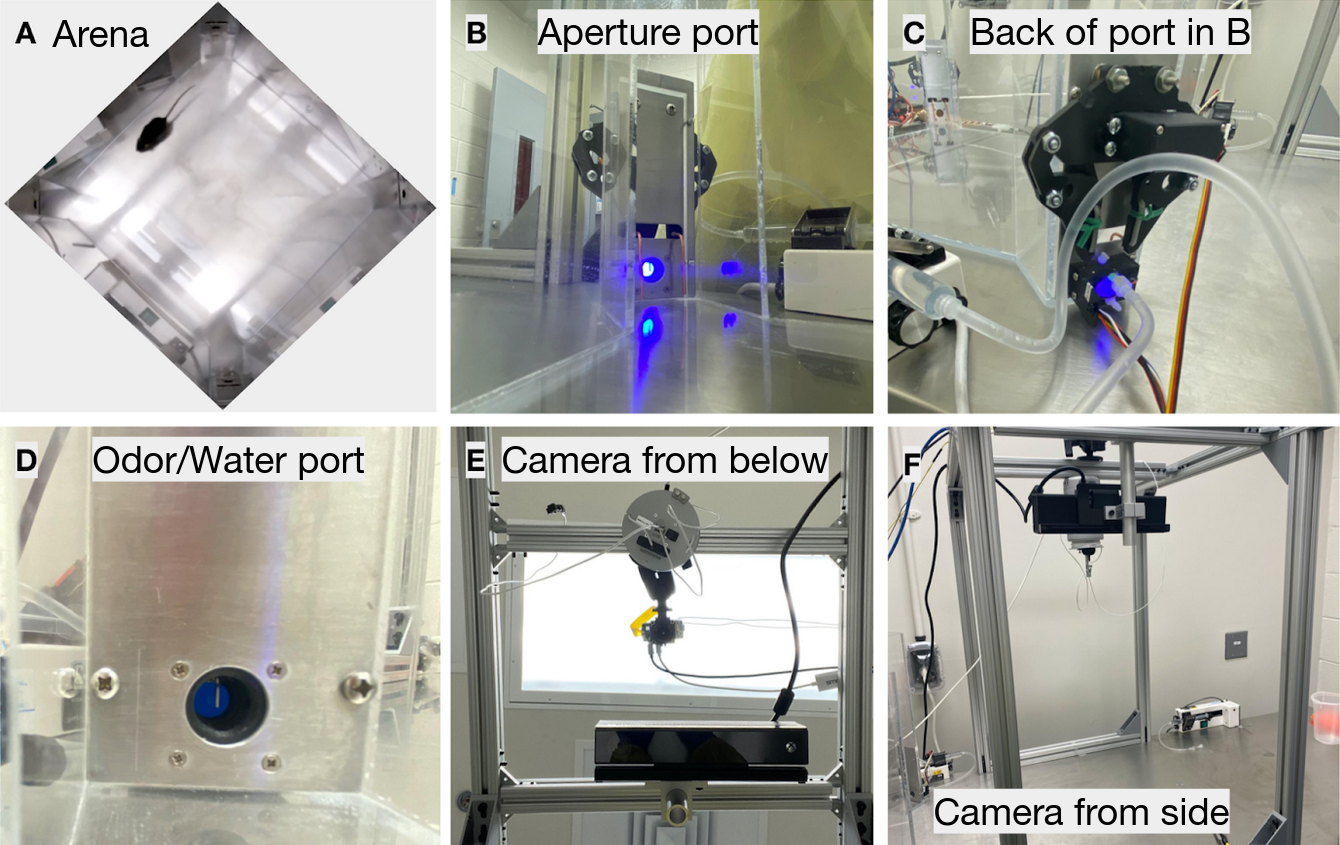
\includegraphics[width=.9\linewidth]{img/physical-diamond-arena.png}
\end{center}
\end{frame}
\section{Hypothesis}
\label{sec:org1249b3c}

\begin{frame}[label={sec:orgdd2c3d9}]{Function approximation}
\begin{columns}
\begin{column}{0.5\columnwidth}
\begin{adjustbox}{max width=\columnwidth, keepaspectratio}
Approximate the value function with a \alert{basis function}~:
\end{adjustbox}
\begin{adjustbox}{max width=\columnwidth, keepaspectratio}
\(\hat{\upsilon}(s, \mathrm{\mathbf{w}}) \: \dot{=} \: \mathrm{\mathbf{w}}^T \mathrm{\mathbf{x}}(s) \: \dot{=} \: \displaystyle\sum_{i=1}^{d}  w_i x_i(s)\)
\end{adjustbox}\\[1em]
\begin{adjustbox}{max width=\columnwidth, keepaspectratio}
\(
  \begin{aligned}
\hat{\upsilon} &: \text{approximate value of state $s$ given weight vector $w$}\\
s &: \text{state}\\
\mathrm{\mathbf{w}} &: \text{$d$-vector of weights underlying the approximate value function}\\
\mathrm{\mathbf{x}} &: \text{vector of features visible when in state $s$}\\
w &: \text{$i$th component of learnable weight vector}\\
x &: \text{$i$th component of vector $x(s)$}\\
  \end{aligned}
\)
\end{adjustbox}
\end{column}
\begin{column}{0.5\columnwidth}
\center
\scriptsize
Find some candidate patterns in the data~: place cells, grid cells~?
\normalsize
\begin{center}
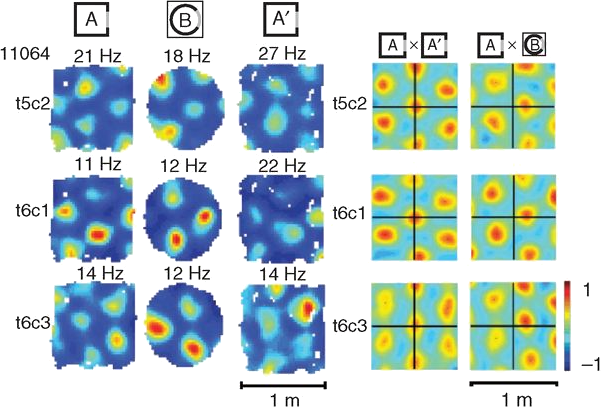
\includegraphics[height=0.25\textheight]{img/place-cells-grid-cells.jpg.png}
\end{center}

\center
\scriptsize
Approximate with coarse coding ? Tiling ?
\normalsize
\begin{center}
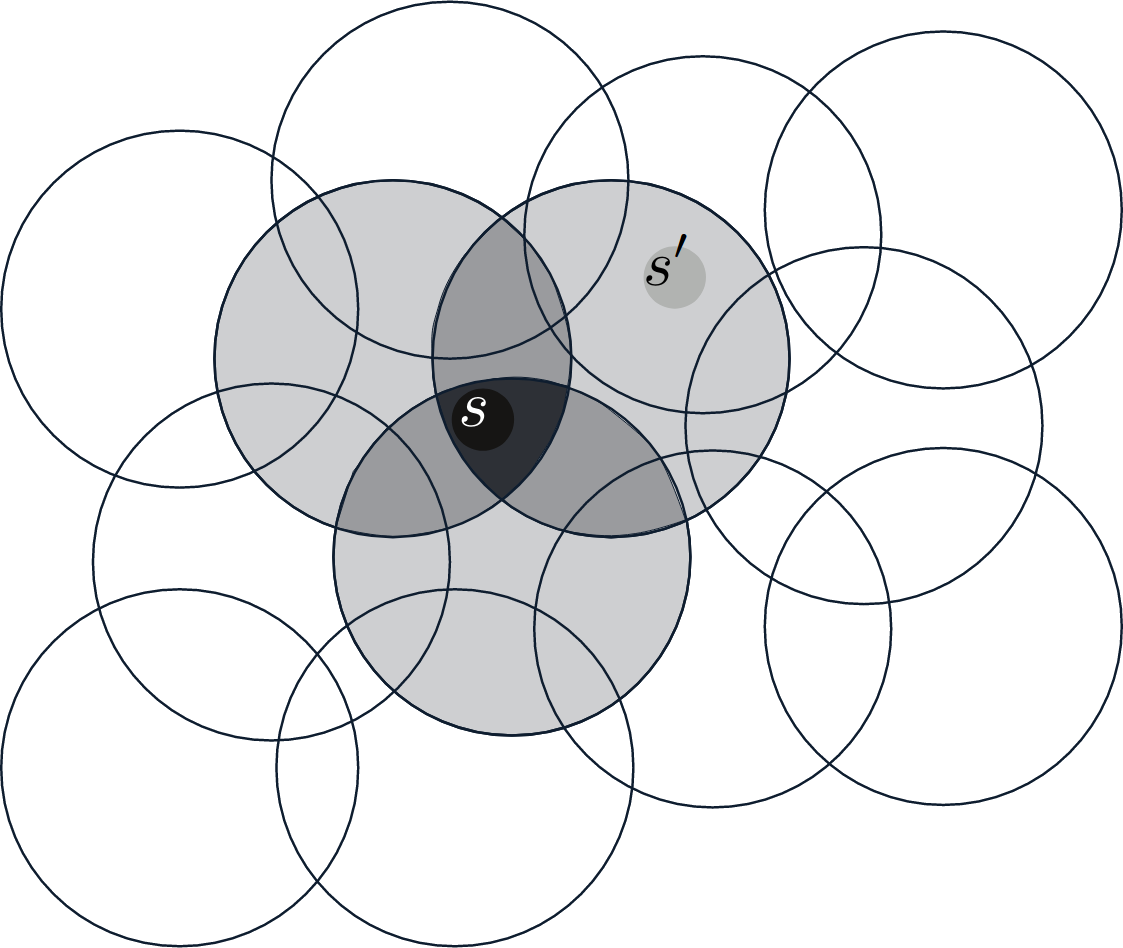
\includegraphics[height=0.25\textheight]{img/coarse-coding.png}
\end{center}

\begin{textblock}{5}(0,12)
\begin{minipage}[t]{3em}
\center
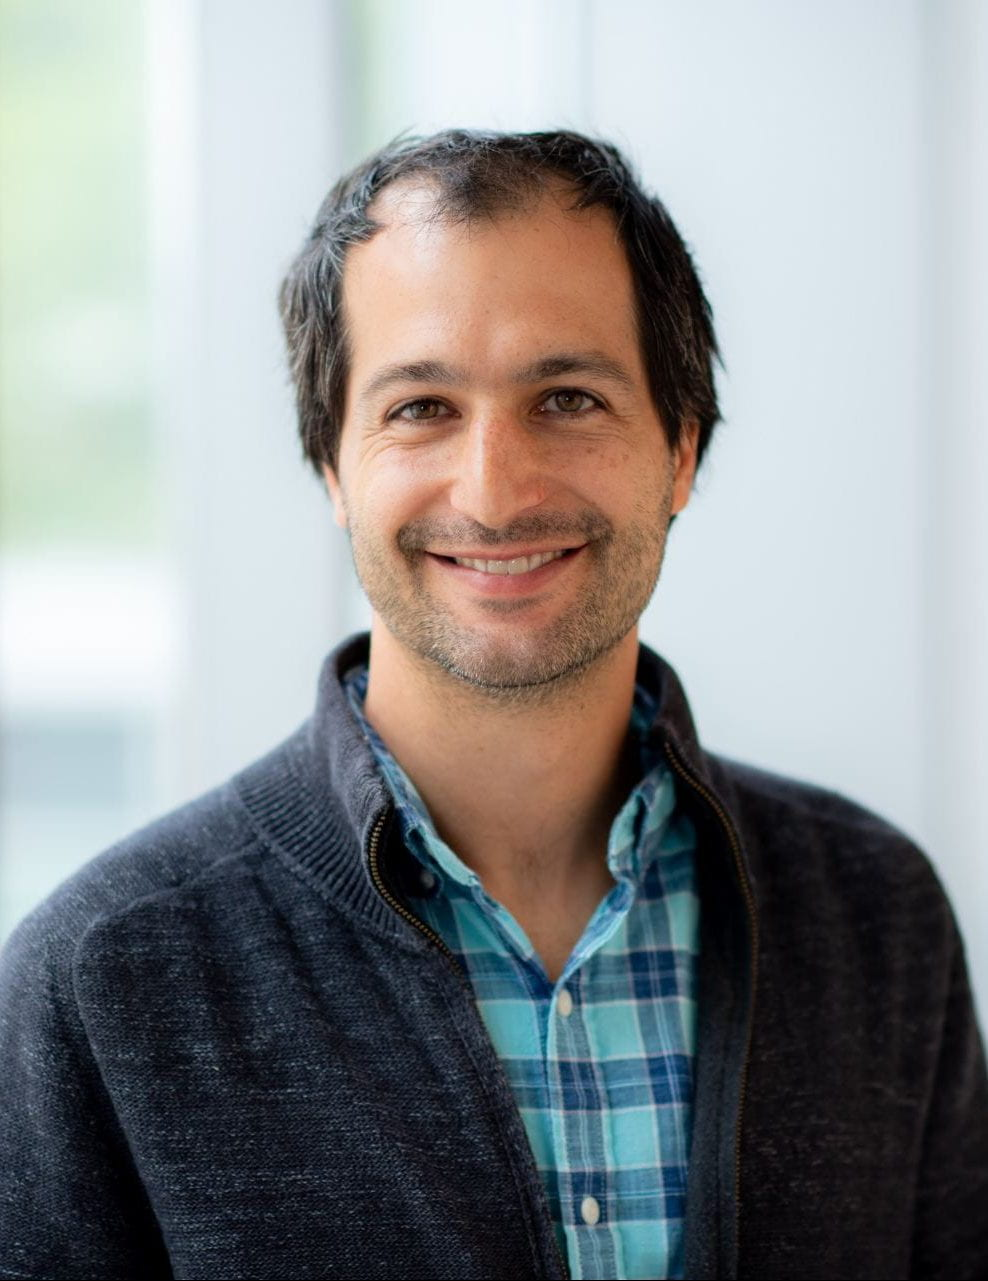
\includegraphics[height=2em]{img/matt-nassar.jpg}\\
\scriptsize
Matt Nassar
\end{minipage}
\begin{minipage}[t]{3em}
\center
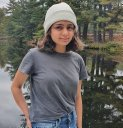
\includegraphics[height=2em]{img/niloufar-razmi.jpeg}\\
\scriptsize
Niloufar Razmi
\end{minipage}
\end{textblock}
\end{column}
\end{columns}
\end{frame}

\section{RL concepts}
\label{sec:org9b35afe}

\begin{frame}[label={sec:org16423ef}]{Temporal Difference learning}
\begin{columns}
\begin{column}{0.5\columnwidth}
\begin{center}
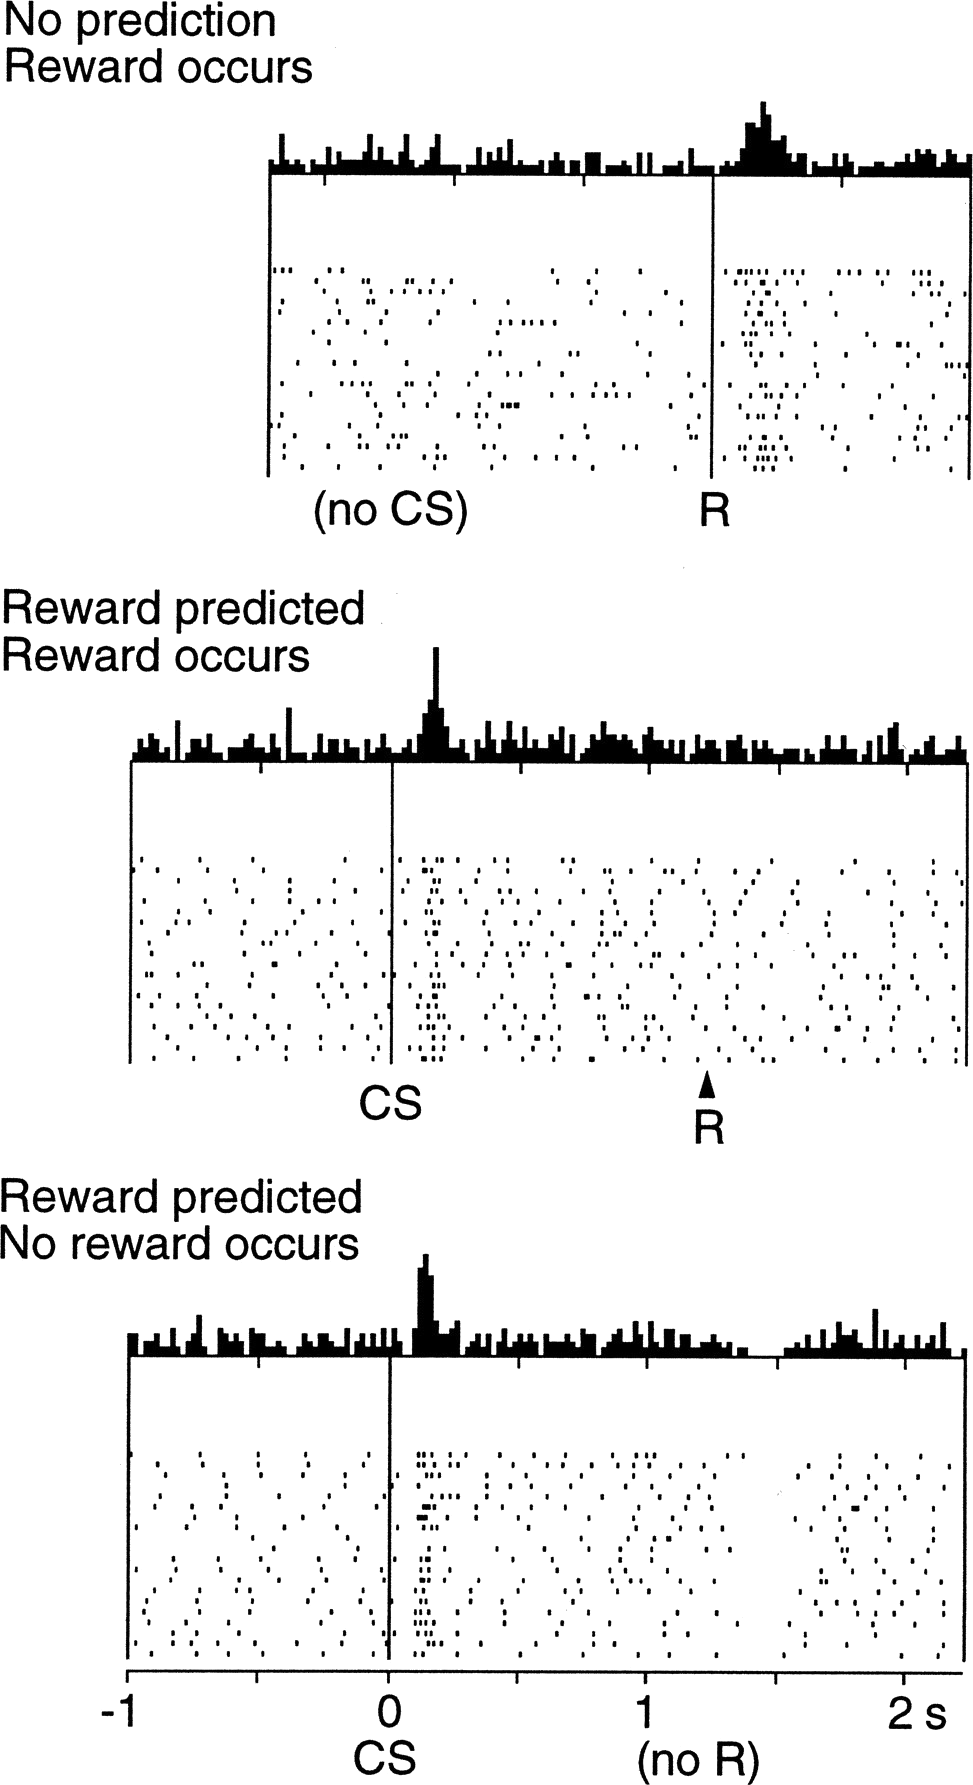
\includegraphics[height=0.8\textheight]{./img/Schultz et al. (1997).png}
\end{center}
Schultz et al. (1997)
\end{column}
\begin{column}{0.5\columnwidth}
\begin{adjustbox}{max width=\columnwidth, keepaspectratio}
$V(S_t) = V(S_t) + \alpha(\underbrace{R_{t+1} + \gamma V(S_{t+1})}_\text{TD target} - V(S_t))$
\end{adjustbox}\\[1em]
\begin{adjustbox}{max width=\columnwidth, keepaspectratio}
$NewEstimate \leftarrow OldEstimate + StepSize[Target - OldEstimate]$
\end{adjustbox}
\end{column}
\end{columns}
\end{frame}
\begin{frame}[label={sec:orgd937368}]{What we're trying to model}
\end{frame}
\begin{frame}[label={sec:org171b9c9}]{General goal}
\end{frame}
\section{Preliminary results}
\label{sec:org9b3b1e7}
\begin{frame}[label={sec:org04f5d8b}]{What did we learn at this point?}
\end{frame}
\section{Experiments}
\label{sec:org4d32dac}
\begin{frame}[label={sec:orge3ad803}]{Split data in 2, learn on first half, predict on second half}
\end{frame}
\begin{frame}[label={sec:org4514429}]{With/without joint repr}
\end{frame}
\section{What we plan to do next}
\label{sec:org238e928}
\begin{frame}[label={sec:org6388b9f}]{What we expect to see}
\end{frame}
\section{Summary}
\label{sec:org110084b}
{%
\setbeamertemplate{background canvas}{\includegraphics[height=\paperheight]{img/grand-canyon.JPG}}
\begin{frame}[fragile,t]{Acknowledgments}
    \begin{columns}[T]
        \begin{column}{0.5\textwidth}
            \begin{itemize}
                \small
                \item Fleischmann lab~:
                \begin{itemize}
                    \tiny
                    \item \textbf{Alexander Fleischmann}
                    \item Simon Daste
                    \item Max Seppo
                    \item Wilson Andrés Mena Orostica
                    \item \colorbox{white}{\transparent{0.2}Sara Zeppilli}}
                    \item Zach Levin
                    \item Robin Attey
                    \item Keeley Baker
                    \item Olivia Mckissick
                    \item Diego Rodriguez
                    \item Shaun Kohli
                    \item Andrew Aoun
                    \item Eseosa Uwaifo
                    \item Erin Meyers
                \end{itemize}
            \end{itemize}
        \end{column}

        \begin{column}{0.5\textwidth}
            \begin{itemize}
                \small
                \item Collaborations~:
                \begin{itemize}
                    \tiny
                    \item \textbf{Jason Ritt} (Carney Institute, Brown University)
                    \item \textbf{Richard Gerkin} (Arizona State University)
                    \item \textbf{Matt Nassar} (Brown University)
                    \item Niloufar Razmi (Brown University)
                \end{itemize}
            \end{itemize}
        \end{column}
    \end{columns}
\end{frame}
}
\begin{frame}[label={sec:orgaa27d36}]{Acknowledgments}
\begin{columns}
\begin{column}{0.5\columnwidth}
\begin{itemize}
\item Alexander Fleischmann
\item Sara Zepilli
\item Max Seppo
\item Olivia McKissick
\item Simon Daste
\item Keeley Baker
\item Nell Klimpert
\item Tuan Pham
\item Camille Donoho
\item Erin Meyers
\item Eseosa Uwaifo
\item Timothy Pyon
\end{itemize}
\end{column}

\begin{column}{0.5\columnwidth}
\begin{itemize}
\item Jason Ritt
\item Matt Nassar
\item Niloufar Razmi
\end{itemize}
\end{column}
\end{columns}
\end{frame}
\begin{frame}[label={sec:orga70b2ac},standout]{~}
Questions ?
\end{frame}
\end{document}
